\documentclass{article}

\usepackage[margin=1.2in]{geometry}
\usepackage[parfill]{parskip}
\usepackage{titlesec}
\usepackage{amsmath}
\usepackage{amsfonts}
\usepackage{fancyhdr}
\usepackage{listings}
\usepackage{graphicx}
\usepackage{hyperref}
\usepackage{algorithmicx}
\usepackage{algpseudocode}

\usepackage{tikz}
\usetikzlibrary{automata}
\usetikzlibrary{arrows}
\usetikzlibrary{arrows.meta}
\usetikzlibrary{decorations, decorations.pathreplacing, shapes}
\usetikzlibrary{calc}

\tikzset{
	%	vertex/.style={circle,draw,minimum size=1.5em},
	%	main node/.style={circle,draw,font=\sffamily\Large\bfseries},
	%	main node/.style={circle,thick,draw},
	edge/.style={->,> = latex'}
}

\tikzset{
	dot/.style={fill, draw, circle, minimum width=10pt, inner sep=0pt, scale=0.3}
}

\title{Thesis Project -- Demo Outline}
\author{Joseph Spearritt}

\pagestyle{fancy}
\lhead{Thesis Project -- Demo Outline}
\rhead{Joseph Spearritt}
\cfoot{\thepage}

\setcounter{secnumdepth}{3}

\titleformat{\paragraph}
{\normalfont\normalsize\bfseries}{\theparagraph}{1em}{}
\titlespacing*{\paragraph}
{0pt}{3.25ex plus 1ex minus .2ex}{1.5ex plus .2ex}

\newcommand{\keyword}[1]{\;\text{\textbf{#1}}\;}

\begin{document}
%	\setlength{\parindent}{0pt}
	
	\begin{itemize}
	
	\item Background/Intro
	
	\begin{itemize}
		
		\item IF vs Access Control (simple example)
		
		\item MAC / Lattice
		
		\item Non-interference
		
		\item Declassification
		
	\end{itemize}

	\item Project Purpose
	
	\begin{itemize}
		
		\item Is IF viable and useful?
		
		\item Specifically: compare the two most mature IF languages -- JIF and Paragon
		
		\item Are either viable in practice? If not, what would they need? Is one more useful than the other?
		
	\end{itemize}
	
	\item Case Studies \& Findings
	
	\begin{itemize}
		
		\item Overview: Battleships, Conference Management, Calendar Scheduler
		
		\item Battleships: declassification
		
		\begin{itemize}
			
			\item Straightforward declassification of coordinates via special query method
			
			\item Easily representable in both JIF/Paragon
			
			\item Example
			
		\end{itemize}
	
		\item Conference Management: timed release
		
		\begin{itemize}
			
			\item Stateful by necessity
			
			\item Easy in Paragon, needs simulation in JIF (loses type safety)
			
			\item Example
			
		\end{itemize}
	
		\item Calendar scheduler: quantification
		
		\begin{itemize}
			
			\item Requires meetings `owned' by a runtime list of users
			
			\item JIF falls over completely, Paragon gets close but the compiler cannot properly infer
			
			\item Example?
			
		\end{itemize}
		
	\end{itemize}
	
	\item Challenges
	
	\begin{itemize}
		
		\item Research languages whyyy
		
		\item Difficult to just get compilers running -- (ultimately developed toolchain to help)
		
		\item Conceptually quite difficult -- not policy agnostic so constantly have to think about the policy in code; I think I understand it \textit{now}... after 9 months
		
		\item Lack of compiler maturity: when have you done something wrong, and when has the compiler just broken?
		
	\end{itemize}

	\item Conclusion
	
	\begin{itemize}
		\item IF ideas are quite useful: it's often not well thought about
		
		\item Neither JIF nor Paragon presents a viable implementation in their current states
		
		\item Paragon's model seems more likely to lead to a production viable system (more flexible/powerful, easier to learn)
	\end{itemize}
	
\end{itemize}

\newpage

DIAGRAMS:

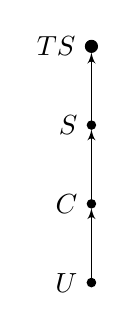
\begin{tikzpicture}
\node[dot, label=left:$ TS $] (TS) at (0, 3) {TS};
\node[dot, label=left:$ S $] (S) at (0, 2) {S};
\node[dot, label=left:$ C $] (C) at (0, 1) {C};
\node[dot, label=left:$ U $] (U) at (0, 0) {U};

\draw[edge] (S) to (TS);
\draw[edge] (C) to (S);
\draw[edge] (U) to (C);
\end{tikzpicture}

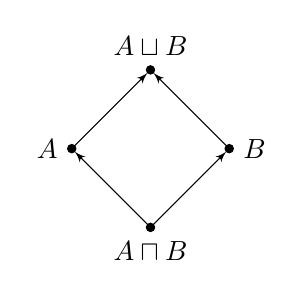
\begin{tikzpicture}
\node[dot, label=above:$ A \sqcup B $] (AuB) at (0, 2) {};
\node[dot, label=left:$ A $] (A) at (-1, 1) {};
\node[dot, label=right:$ B $] (B) at (1, 1) {};
\node[dot, label=below:$ A \sqcap B $] (AnB) at (0, 0) {};

\draw[edge] (AnB) to  (A);
\draw[edge] (AnB) to  (B);
\draw[edge] (A) to  (AuB);
\draw[edge] (B) to  (AuB);
\end{tikzpicture}
	
\end{document}